

\documentclass[a4paper]{scrartcl}

\usepackage{graphicx} % Required for the inclusion of images
\usepackage{xcolor}
\usepackage{epstopdf}
\usepackage{hyperref}


\title{User Rating Based Comparison of Tone Mapping Operators for HDR Images \\ Multimedia Communications AS 2015} %Title

\author{Taivo Pungas \\ 15-928-336} % Author name

\date{\today} % Date for the report

\begin{document}

\maketitle % Insert the title, author and date


\section{Introduction}
\subsection{Motivation}

Most classified ads -- ranging from real estate to used guitars -- contain images. In most cases these images are taken by non-experts, and even when a professional photographer is used, photos might not reflect the advertised object accurately; one possible cause is the low dynamic range (LDR) of the images.

Assuming the look and feel of images play an important part in buying decisions, we naturally get to the questions: do scenes or objects depicted in high dynamic range (HDR) images look better compared to LDR images? Which tone mapping operator (TMO) gives the best result?


\subsection{Approach}

I will:
\begin{enumerate}
	\item Create HDR images by combining multiple images taken at different exposures and tone-map the images using a Matlab toolbox\footnote{\url{https://github.com/banterle/HDR_Toolbox}} from \cite{Banterle:2011}.
	\item In a survey, ask users how pleasant they find the images.
	\item Compare the results of LDR images and different TMOs for HDR images.
\end{enumerate}

\subsection{Expected Outcome}

I will rank different TMOs and compare them with LDR images. I will compare the results for different lighting conditions.

\section{Theoretical Background}

\subsection{HDR images}

The luminance of a region of an image describes the intensity of light originating from that region and captured in the camera sensor.

A scene can be said to have high dynamic range if the amount of light is very high in some regions and very low in others. Standing in a dark room during the day and looking towards a window is an example of a high dynamic range scene: a lot of light is coming from the window but very little from the surrounding walls.

The dynamic range of a camera [monitor] is a measure of the range of luminance values that can be captured [displayed] using the device. The dynamic range of typical commercial cameras is low, which means it is hard to capture details in both light and dark areas of the image. Furthermore, even if an HDR image can be captured (e.g. by merging images taken at different exposure values), most monitors are unable to display a high dynamic range of values (i.e. HDR images can not be reproduced as-is on these monitors).

\subsection{Tone mapping operators}

We can solve to the problem of reducing a large range of luminance values (from the HDR image) to a small range (the capability of monitors) by mapping the large range to the small range using a \emph{tone mapping operator} (TMO). "This reduction of the range attempts to keep some characteristics of the original content such as local and global contrast, details, etc. Furthermore, the perception of the tone mapped image should match the perception of the real-world scene." \cite{Banterle:2011}

Having multiple criteria implies multiple optimisation goals and so we should expect that there is no single optimal solution; rather, choosing a TMO involves some amount of artistic liberty. The goal of this work is to find the TMO that is considered aesthetically most pleasing by users.

\section{Implementation and pipeline}
\label{sec:implementation}

The end-to-end pipeline of selecting images for surveys was as follows:
\begin{itemize}
\item Capture 40 scenes. For each scene, three images were taken: one with automatic settings chosen by the camera (Olympus E-400) and two others with exposure values (EV) -1 and +1 using automatic exposure bracketing (AEB). The images were taken in Tallinn, Estonia, during dusk of December 19, 2015. All images were taken using a camera stand to avoid shift in the scenes.
\item Choose 4 scenes out of the 40 so that the scenes would be dissimilar in composition, without ghosting, and without motion blur (due to camera movement).
\item Resize images from 3648x2736 to 1067x800 to speed up HDR image generation and tone-mapping.
\item Create HDR image for each scen using the three AEB images.
\item Run all 27 available TMOs in the toolbox \cite{Banterle:2011} with their default parameters (which are set to values recommended by the TMOs' original authors).
\item Apply gamma correction to tone-mapped images where necessary.
\item Pick top 4 TMOs to compare in the user survey such that the TMOs produce images that are visually different enough and don't have gross aesthetic failures (e.g. extremely low brightness). The chosen TMOs were Drago \cite{drago2003adaptive}, Kuang \cite{kuang2007icam06}, Mertens \cite{mertens2007exposure} and WardHistAdj \cite{larson1997visibility}.

\end{itemize}

This process yielded 16 images: one for each TMO-scene pair. \\

\paragraph{Code} The implementation can be found in the folder \texttt{code}: 

\begin{itemize} 

\item \verb+pipeline.m+ runs the pipeline from generating HDR images to mapping them to LDR images using TMOs.
\item \verb+build_hdrs.m+ creates HDR images from given sets of LDR images taken at different exposures.
\item \verb+build_comparison.m+ creates a single tiled image of all tone images compared in this work for easy visual comparison.

\end{itemize}

\paragraph{Images} All images can be found in the folder \texttt{images}.

\begin{itemize}

\item \texttt{combined.jpg} is a tiled image of all tone-mapped images compared in this work.
\item \verb+combined_all.jpg+ is a tiled image of all tone-mapped images generated, including ones not shown to users in the survey.
\item \verb+best_worst.jpg+ is a comparison of the best and worst tone-mapped images according to the user ratings.
\item Folders \texttt{kalamaja2}, \texttt{niguliste}, \texttt{ptln1}, and \texttt{toompea4} each contain the files for one scene:
	\begin{itemize}
	\item \verb+PC*.JPG+, the three images taken using AEB.
	\item \verb+hdr_image.pfm+, the HDR image generated from this scene.
	\item \verb+tmo__Original.JPG+, the image taken using automatic settings chosen by the camera.
	\item \verb+tmo_<name>.jpg+, the tone-mapped images, where \texttt{<name>} is the name of the TMO used.
	\end{itemize}

\end{itemize}

\newpage
\section{Experiments and Results}

\subsection{Survey method}

In the user survey, each user was presented with five images for each scene: four tone-mapped images from the HDR-TMO pipeline, plus the original image captured with automatic camera settings. The images were presented in a fixed order that was the same for all respondents. This yielded a total of 20 images for each user to rate; I chose such a low number of TMOs and scenes since I expected a sample of less than 50 users. Figure~\ref{fig:tiled_tmo_images} shows all the images included in the survey.

Each image was shown on a separate page and the user was asked to evaluate each image for individual aesthetic merit, not compare it with previous images. The user was asked "How much do you like the following image?" and the answers were given on a Likert scale ranging 1 to 7 with integer steps. A rating of 1 corresponded to "Do not like at all", 4 to "Neutral" and 7 to "Like very much".

The survey was implemented using Google Forms and conducted in Estonian as the primary audience were Estonians. I acquired 126 participants by individually inviting (roughly 20 respondents) and sharing the questionnare on my Facebook page (roughly 100 respondents). Each of the 126 participants gave a total of 20 ratings yielding a total of 2520 ratings. 

\subsection{Results}

From Figure~\ref{fig:line_meanrating_vs_scene}, we can see that there is no TMO that always performs better than others, however Mertens and Drago perform worse in all scenes than Kuang and WardHistAdj. The same is visible from the rating distributions on Figure~\ref{fig:bar_histogram_tmo} and on Figure~\ref{fig:bar_histogram_tmo_scene}: Drago and Mertens are rated consistently lower. In interpreting the data, it is important to note that Toompea4 was a much darker scene than others -- this shows in the data as clearly the performance of all TMOs is low on that scene.

When we compare the TMOs' ratings with those of the original images, we see a very uneven performance: The original images rank first on two scenes (significantly so in the scene Niguliste), fourth on one scene and second/third on one scene.

For ease of reference, the best and worst images for each scene are shown in Figure~\ref{fig:best_worst_images}.


\begin{figure}[h]
\centering
\includegraphics[width=1\textwidth]{figures/line_meanrating_vs_scene.pdf}
\caption{Mean user ratings by scene and TMO.}
\label{fig:line_meanrating_vs_scene}
\end{figure}

\begin{figure}[h]
\centering
\includegraphics[width=1\textwidth]{figures/bar_histogram_tmo.pdf}
\caption{Distribution of ratings by TMO}
\label{fig:bar_histogram_tmo}
\end{figure}

\begin{figure}[p]
\centering
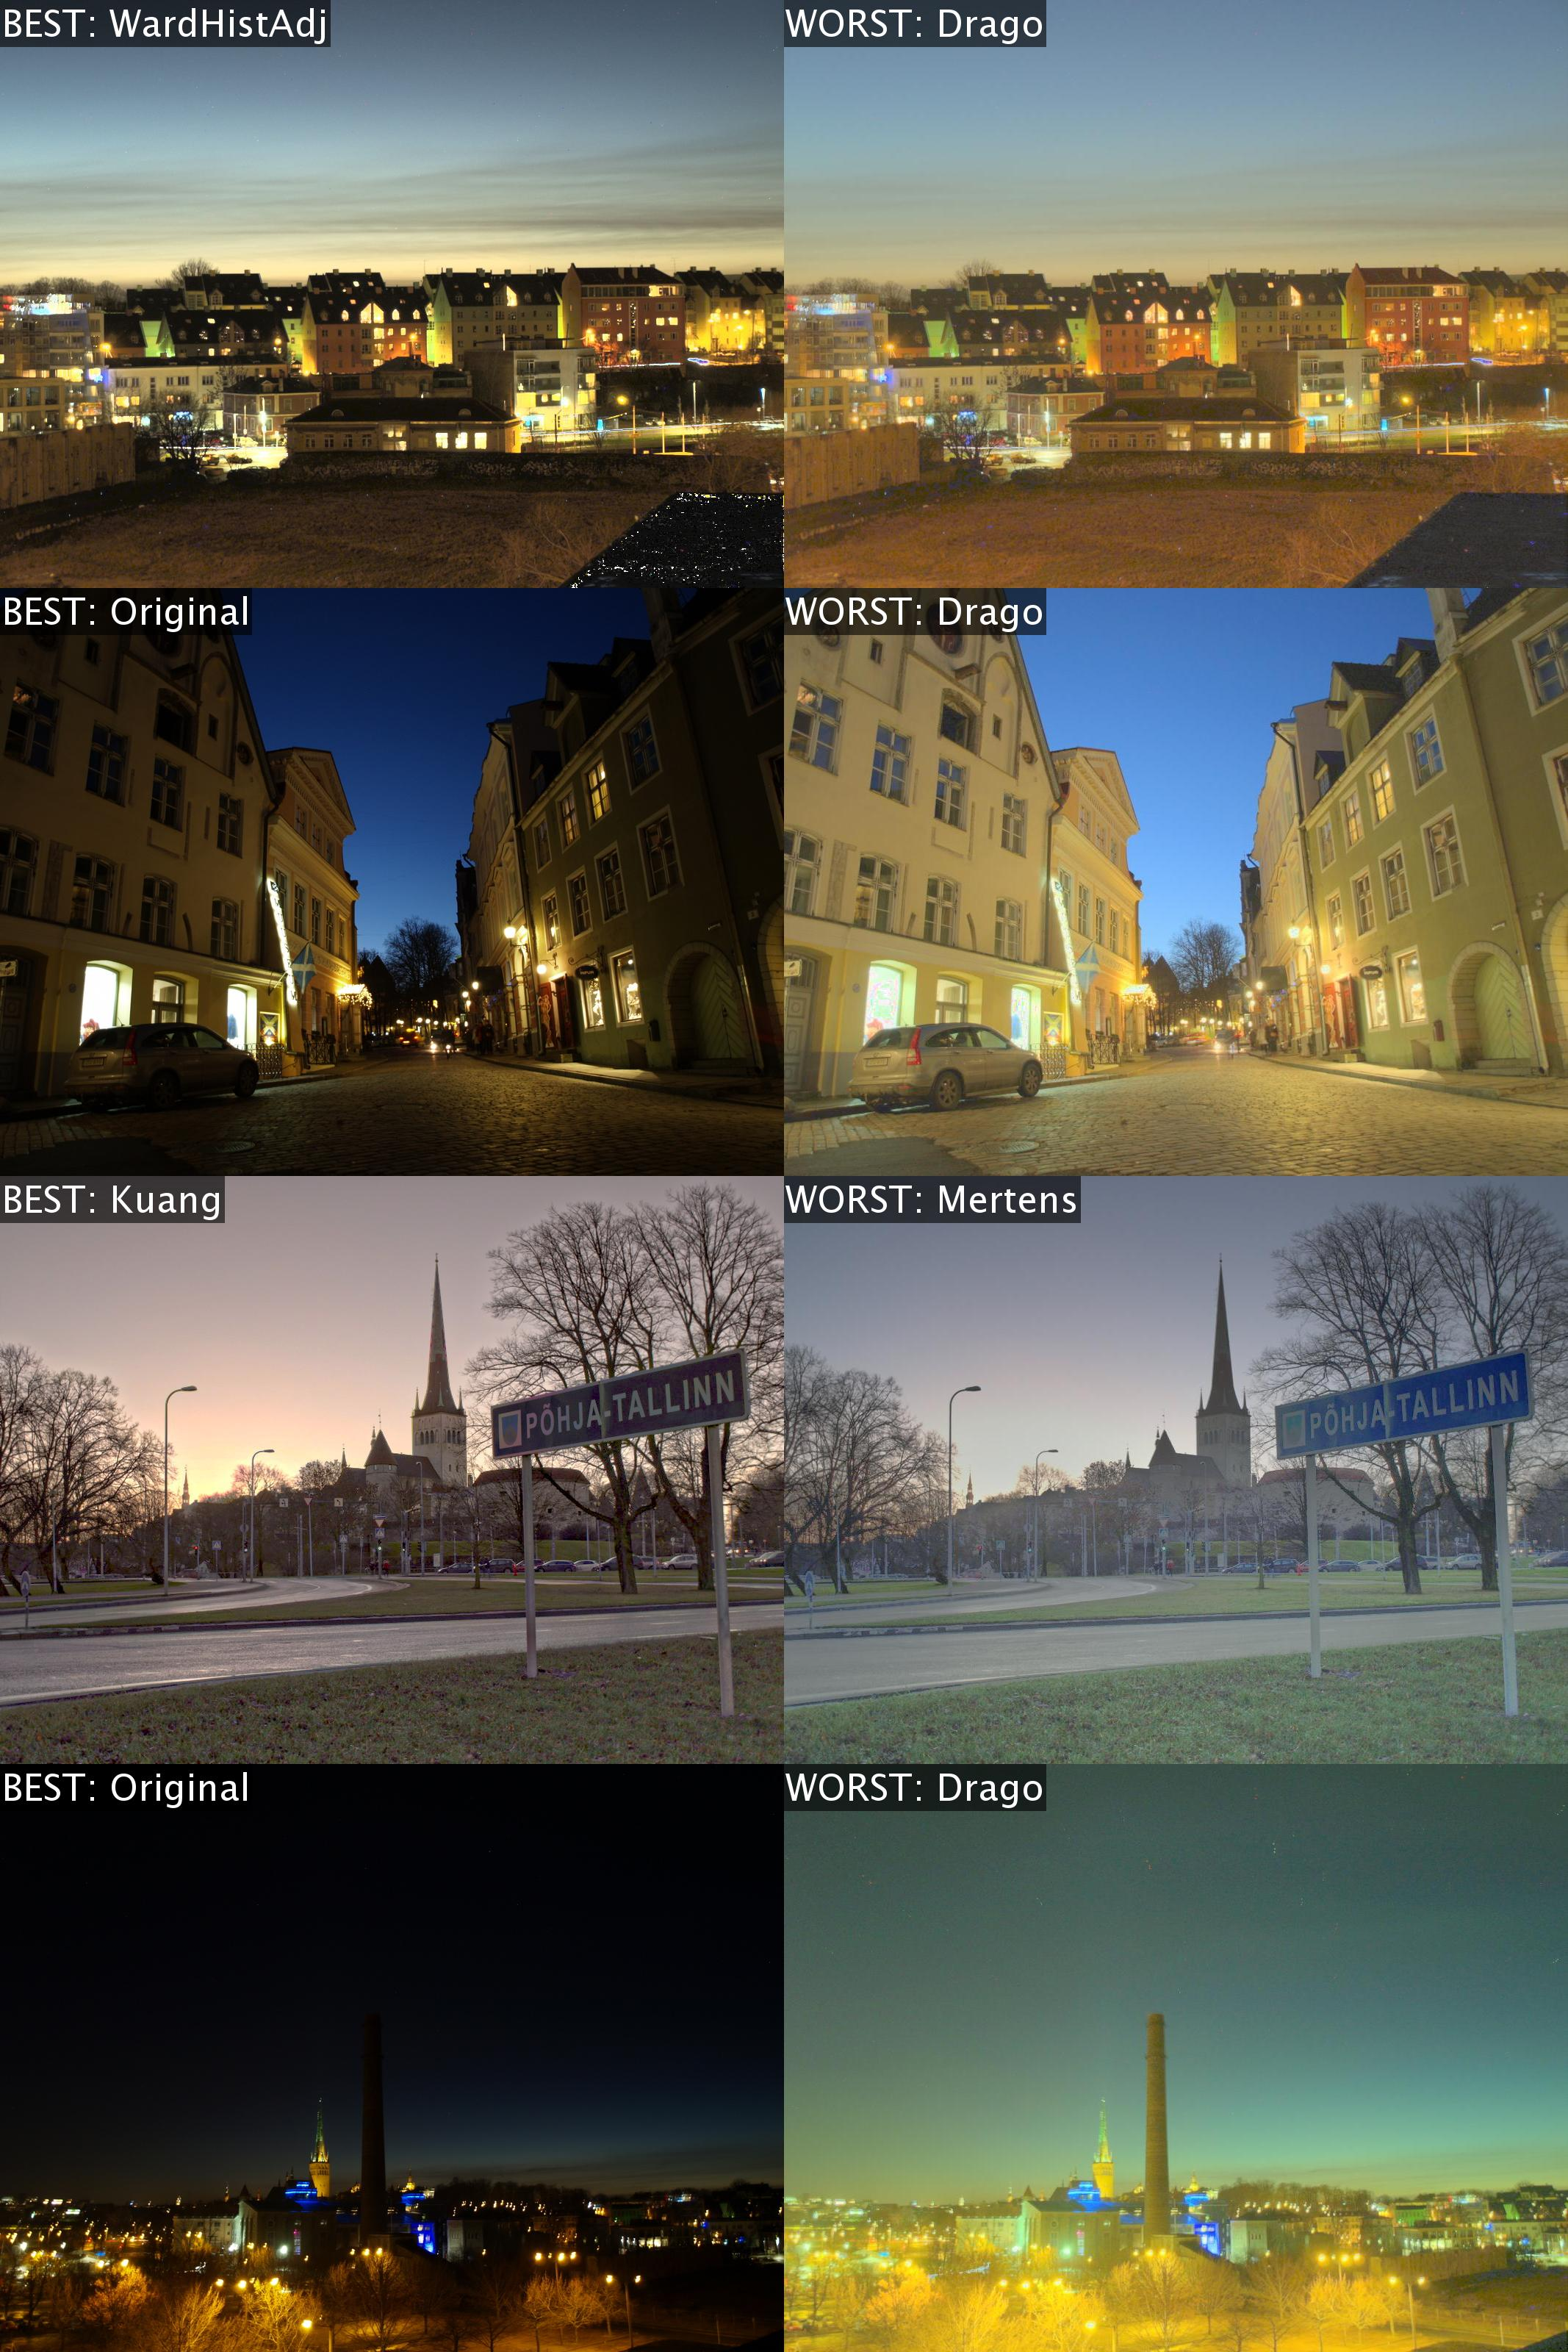
\includegraphics[width=0.9\textwidth]{../images/best_worst.jpg}
\caption{The best and worst tone-mapped images according to user ratings.}
\label{fig:best_worst_images}
\end{figure}

\section{Discussion} 


Given that Kuang is better than all other TMOs in all images but one and delivers consistent performance across all images, I would rank it above WardHistAdj. Mertens also beat Drago in all images but one and was more consistent in aesthetic quality, so from the results of this survey, I would rank the TMOs as:

$$\textrm{Kuang} > \textrm{WardHistAdj} > \textrm{Mertens} > \textrm{Drago}$$

Given that the aesthetic performance of the original images is highly uneven but beats all TMOs in some cases, I recommend considering the original image as an option if the goal is to select the most visually pleasing image. It is also interesting that the original image performs relatively better whenever the scene is dark (Niguliste and Toompea4) -- this can be taken into account in an automated image aesthetics improvement algorithm like the one proposed in \cite{aydin2015automated}.

\paragraph{Room for improvement}

There are several features of this study that could be improved upon. First, increasing the user sample size would allow making stronger statements about more scenes and more TMOs, which would allow us to make more general statements about the relative aesthetic performance of TMOs.

Second, image presentation order in the user survey should be randomised to remove undesired effects caused by giving all users a baseline (the image that was first shown).

Third, users may be better at comparing pairs of images rather than rating images in isolation. One way to achieve this would be to use the Elo rating system (as a colleague pointed out to me in an informal chat).

Fourth, the TMO parameters should also be varied. In the current study, the performance of some TMOs may have been hindered by a suboptimal choice of parameters. This, however, would need a much larger sample size or automated image aesthetics analysis.


\section{Summary and conclusion}

In this study, I compared how different TMOs are rated by users. I proposed a user-rating-based ranking of TMOs and found that the original (i.e. LDR) image may significantly outperform tone-mapped HDR images, especially in low-light conditions where all TMOs perform worse than in better-lit scenes.

\newpage\bibliographystyle{unsrt}

\bibliography{report}


\newpage\section*{Appendix A: distribution of ratings by TMO and scene.}
\begin{figure}[h!]
\centering
\includegraphics[width=1\textwidth]{figures/bar_histogram_tmo_scene.pdf}
\caption{Distribution of ratings by TMO and scene.}
\label{fig:bar_histogram_tmo_scene}
\end{figure}


\newpage\section*{Appendix B: all images shown to users.}
\begin{figure}[h!]
\centering
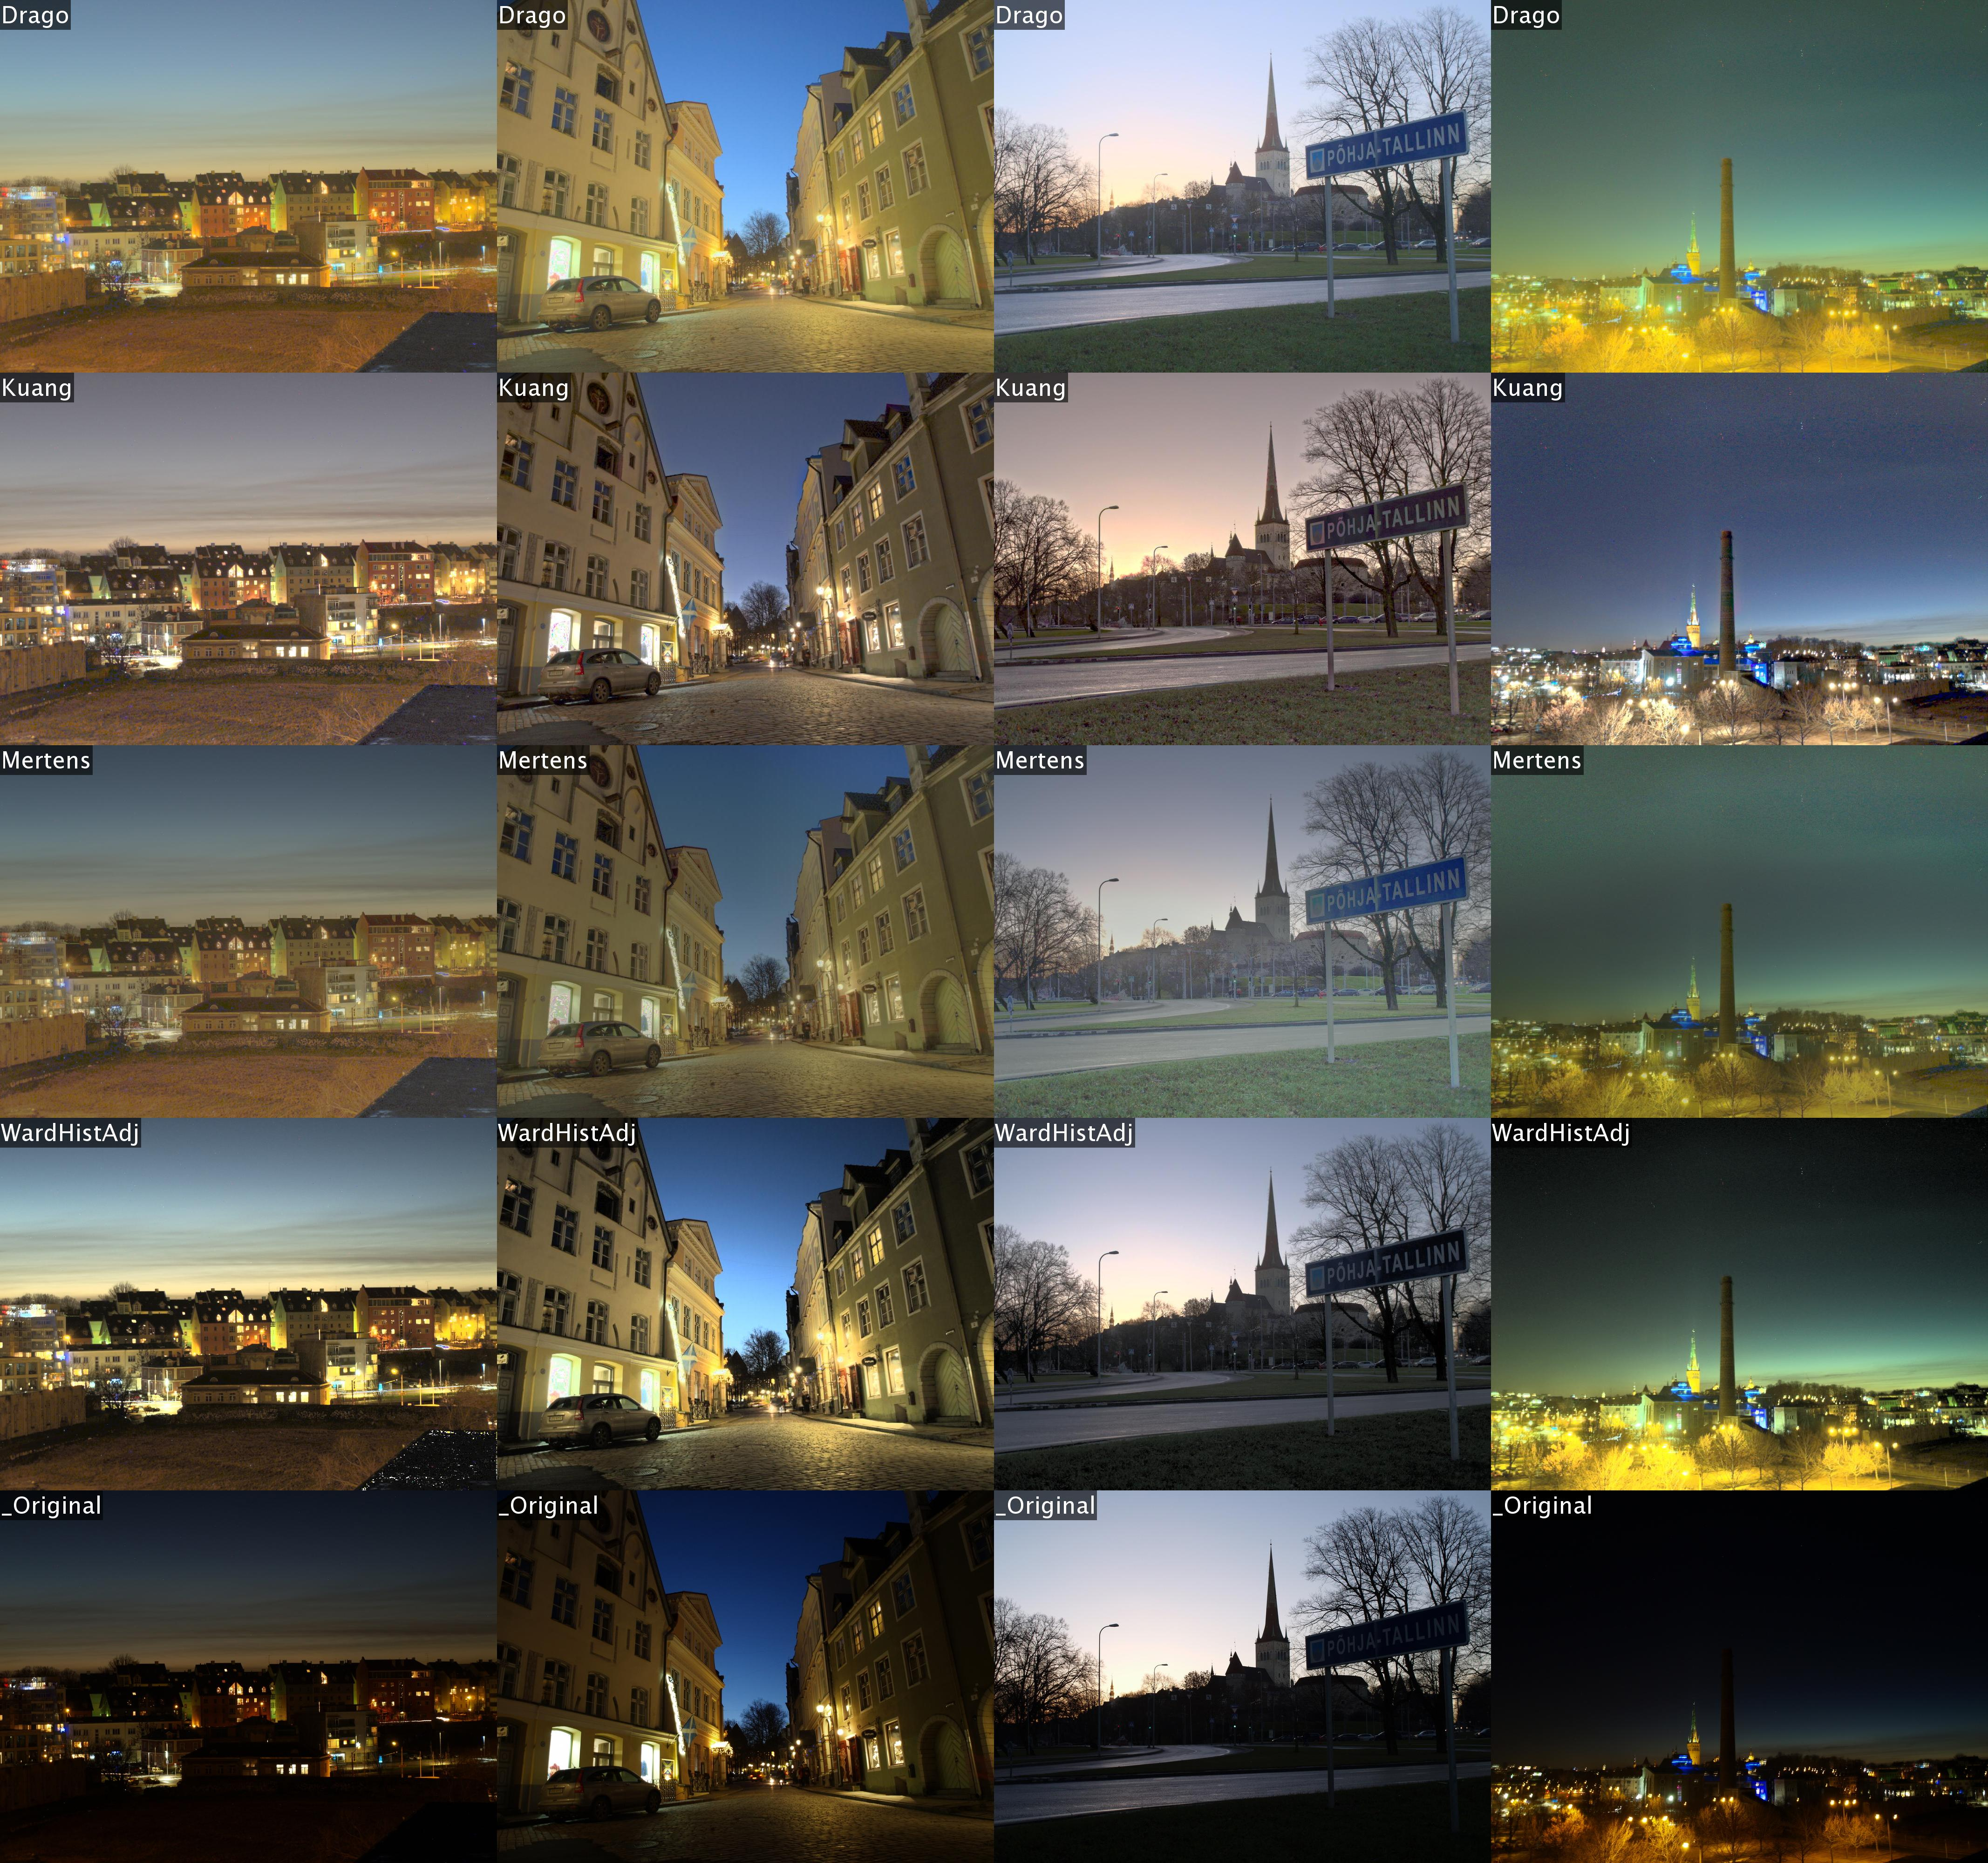
\includegraphics[width=1\textwidth]{../images/combined.jpg}
\caption{Tone-mapped images (top 4 rows) and the original image taken with automatic settings (bottom row).}
\label{fig:tiled_tmo_images}
\end{figure}


\end{document}
